\documentclass[aspectratio=169]{beamer}

\usetheme{Madrid}
\usecolortheme{DSLAB}
\usefonttheme[onlylarge]{structurebold}
\setbeamerfont*{frametitle}{size=\normalsize,series=\bfseries}
\setbeamertemplate{navigation symbols}{}

\usepackage[utf8]{inputenc}
\usepackage[T1]{fontenc}
\usepackage[spanish]{babel}
\usepackage{xmpmulti}
\usepackage{tikz}
\usepackage{pgf}
\usepackage{amsmath}
\usepackage{amsfonts}
\usepackage{graphicx}
\usepackage{color}
\usepackage{multirow}
\usepackage{lmodern}
\usepackage{hyperref}
\usepackage{eurosym}

\usetikzlibrary{arrows,positioning,shapes.geometric}
\tikzstyle{block}=[draw opacity=0.7,line width=1.4cm]

\setbeamercovered{dynamic}
\setbeamerfont{author}{family=\rmfamily}
\institute[URJC]{DSLAB}

\author[Big Data Processing II]{
	Alberto Fernández Isabel \\
	Natalia Madrueño Sierro \\
	Rubén Rodríguez Fernández \\
}

\title[Tema 1: Procesamiento en Entornos Distribuidos]{
	Big Data Processing II \\ \vspace{0.2em}
	\large{Tema 1: Procesamiento de Big Data en Entornos Distribuidos}
}
\date{Febrero 2026}
\titlegraphic{
\includegraphics[width=3cm]{images/logourjceps.png}}

\setbeamertemplate{section page}{
	\vspace{1cm}
	\begin{beamercolorbox}[sep=8pt,center,wd=\textwidth]{section title}
		\usebeamerfont{section title}\insertsection\par
	\end{beamercolorbox}
}

\AtBeginSection[]{
	\begin{frame}
	\frametitle{Contenido}
		\tableofcontents[currentsection,hideothersubsections]
	\end{frame}
}

\begin{document}

\begin{frame}
  \titlepage
\end{frame}

\begin{frame}
\frametitle{Objetivos}
	\begin{itemize}
    \item Comprender la transición del procesamiento \textbf{batch} a \textbf{streaming} en analítica deportiva
    \item Identificar las características de los sistemas de \textbf{mensajería distribuida}
    \item Conocer los fundamentos de los motores de \textbf{procesamiento en tiempo real}
    \item Familiarizarse con los \textbf{principios de diseño} de arquitecturas distribuidas
    \item Relacionar estos conceptos para casos de uso en el \textbf{análisis deportivo en vivo}
	\end{itemize}
\end{frame}

\begin{frame}
\frametitle{Índice}
	\tableofcontents
\end{frame}

\section{Introducción}

\begin{frame}\frametitle{Introducción - Evolución del análisis deportivo}
	\begin{itemize}
		\item \textbf{El análisis de datos puede apoyar la toma de decisiones durante el evento}
		\begin{itemize}
			\item Antes $\Rightarrow$ análisis después del entrenamiento o partido
			\item Ahora $\Rightarrow$ decisiones en vivo sobre táctica, rotaciones y gestión de la carga
		\end{itemize}

		\vspace{1em}

		\item El foco se desplaza de \textbf{datos estáticos} a \textbf{eventos continuos} procesados en tiempo real
	\end{itemize}
\end{frame}


\begin{frame}\frametitle{Introducción - Evolución del análisis deportivo}
	\begin{itemize}
		\item \textbf{El valor del dato deportivo cae con el tiempo}
		\begin{itemize}
      \item Información procesada tarde es una oportunidad perdida
      \item Lo correcto a destiempo puede no ser de utilidad en la práctica
    \end{itemize}

    \vspace{1em}
      
    \item \textbf{Ejemplos de analítica deportiva en vivo}
		\begin{itemize}
			\item Fatiga y lesión, con alertas durante el esfuerzo, no después
			\item Tracking de jugadores, detectando patrones de presión, desmarques y desajustes en vivo
		\end{itemize}
	\end{itemize}
\end{frame}

\begin{frame}
\frametitle{Introducción - Big data tradicional}
	\begin{itemize}
		\item \textbf{Procesamiento de datos en batch}
		\begin{itemize}
			\item Se recopila un conjunto de datos y se analiza después
			\item Se asume que el dataset está completo antes de procesar
		\end{itemize}

		\vspace{1em}

		\item \textbf{Casos de uso en el ámbito deportivo}
		\begin{itemize}
			\item Reporting / scouting, histórico, modelos offline y análisis exploratorio
			\item Presenta una alta latencia, el resultado llega cuando la acción ya terminó
		\end{itemize}
	\end{itemize}
\end{frame}

\begin{frame}
\frametitle{Introducción - Procesamiento en batch}
	\begin{itemize}
		\item \textbf{Se usa un conjunto de datos cerrado y finito}
		\begin{itemize}
			\item Hay un final conocido, se puede procesar todo
			\item \textit{input cerrado} $\rightarrow$ procesamiento $\rightarrow$ \textit{output final}
		\end{itemize}

		\vspace{1em}

    \item \textbf{Optimiza la capacidad global del sistema}
      \begin{itemize}
        \item Throughput $\rightarrow$ cuántos datos se procesan por unidad de tiempo
      \end{itemize}
    
    \vspace{1em}

    \item \textbf{No prioriza el tiempo de respuesta individual}
    \begin{itemize}
      \item Latencia $\rightarrow$ cuánto tarda un evento en producir un resultado
    \end{itemize}
  \end{itemize}
\end{frame}

\begin{frame}
\frametitle{Introducción - Procesamiento en batch}
\begin{center}
	  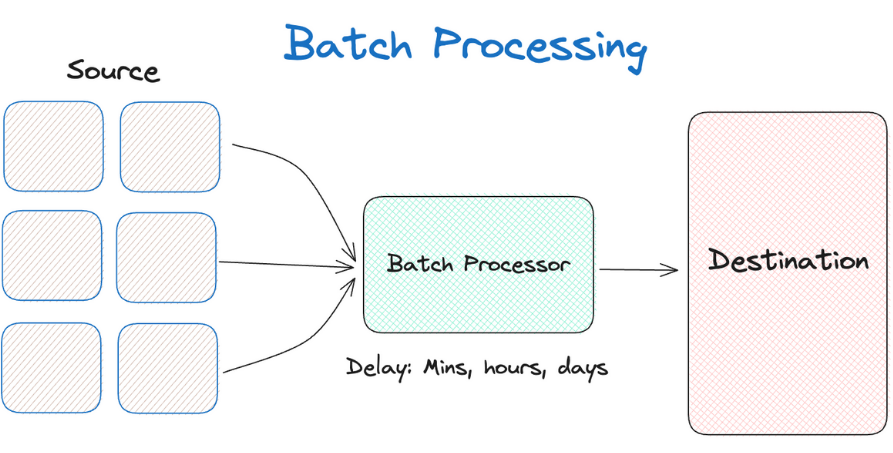
\includegraphics[width=0.8\linewidth]{images/batch.png} \\
    {\fontsize{5}{6}\selectfont \mbox{Fuente: \url{https://www.decube.io/post/streaming-vs-batch-data}}}
\end{center}
\end{frame}

\begin{frame}
\frametitle{Introducción - Procesamiento en batch}
\begin{columns}
	\begin{column}{0.6\textwidth}
		\begin{itemize}
			\item \textbf{Tecnologías habituales}
			\begin{itemize}
				\item Hadoop y MapReduce para grandes lotes distribuidos
				\item Spark batch como API de alto nivel e iteración más rápida
			\end{itemize}

			\vspace{1em}

			\item \textbf{Almacenamiento}
			\begin{itemize}
				\item Data Lakes y Data Ware Houses para almacenar históricos
			\end{itemize}
		\end{itemize}
	\end{column}

	\begin{column}{0.35\textwidth}
		\centering
		
\includegraphics[width=0.8\textwidth]{images/hadoop.png}
		\vspace{1em}

		
\includegraphics[width=0.8\textwidth]{images/spark_batch.png}
	\end{column}
\end{columns}
\end{frame}

\begin{frame}
\frametitle{Introducción - Del big data al fast data}
	\begin{itemize}
		\item \textbf{Big Data se centra en volumen}
		\begin{itemize}
      \item Almacena y procesa grandes volúmenes de datos
      \item Procesamiento en batch analiza datos finitos
      \item Ejemplos incluyen datos históricos deportivos
		\end{itemize}

		\vspace{1em}

    \item \textbf{Fast Data se centra en velocidad}
		\begin{itemize}
      \item Procesa y toma decisiones sobre los datos mientras se generan
      \item Procesamiento en streaming analiza flujos continuos
      \item Ejemplos incluyen datos de tracking en vivo
		\end{itemize}
	\end{itemize}
\end{frame}

\begin{frame}
\frametitle{Introducción - Datos finitos vs continuos}
	\begin{itemize}
		\item \textbf{Datos finitos (bounded)}
		\begin{itemize}
			\item Datos cerrados con fin definido
			\item Se da un único resultado al final
			\item Caso particular de datos continuos
		\end{itemize}

		\vspace{1em}

    \item \textbf{Datos continuos (unbounded)}
		\begin{itemize}
			\item Flujo de datos potencialmente infinito
			\item Hay que producir resultados en continuo
		\end{itemize}
	\end{itemize}
\end{frame}

\begin{frame}
\frametitle{Introducción - Datos fríos y calientes}
	\begin{itemize}
		\item \textbf{La temperatura del dato se refiere a su frescura y utilidad}

		\vspace{1em}

    \item \textbf{Datos fríos (cold)}
		\begin{itemize}
			\item Histórico, auditoría y entrenamiento de modelos
			\item Procesamiento en batch opera sobre frío
		\end{itemize}

		\vspace{1em}

    \item \textbf{Datos calientes (hot)}
		\begin{itemize}
			\item Máximo valor ahora, requieren decisión inmediata
			\item Procesamiento en streaming opera sobre caliente
		\end{itemize}

	\end{itemize}
\end{frame}

\begin{frame}
\frametitle{Introducción - Cambio de paradigma}
	\begin{itemize}

    \item \textbf{Concepto de panta rei o ``todo fluye``}
		\begin{itemize}
      \item La realidad está en cambio continuo
			\item Es una secuencia de eventos con contexto
			\item No se piensa en una tabla final, sino en una historia que se actualiza
		\end{itemize}

		\vspace{1em}

		\item \textbf{Cambio de mentalidad hacia flujos dinámicos de eventos}
	\end{itemize}
\end{frame}

\begin{frame}
\frametitle{Introducción - Procesamiento en streaming}
	\begin{itemize}
    \item \textbf{Computación incremental sobre eventos}
      \begin{itemize}
        \item Se prioriza la velocidad en la toma de decisiones
        \item Procesa eventos conforme llegan, sin esperar a un dataset completo
        \item Genera resultados incrementales que se refinan con cada nuevo evento
		\end{itemize}

		\vspace{1em}

		\item \textbf{Requiere un trade-off entre latencia, coste y exactitud}
	\end{itemize}
\end{frame}

\begin{frame}
\frametitle{Introducción - Procesamiento en streaming}
\begin{center}
	  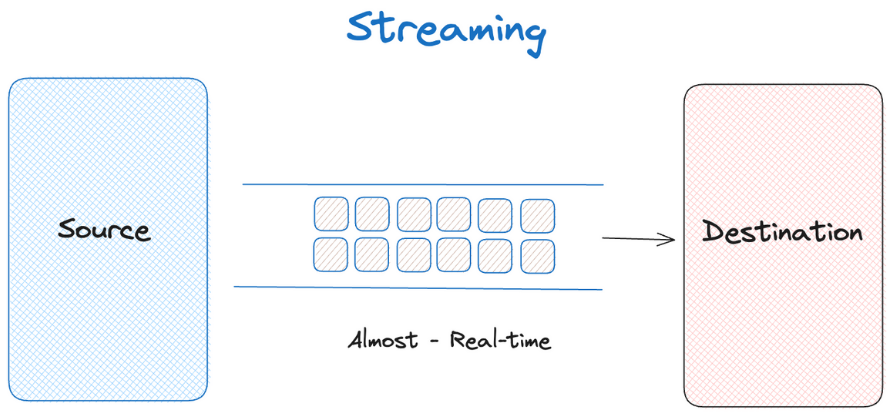
\includegraphics[width=0.8\linewidth]{images/streaming.png} \\
    {\fontsize{5}{6}\selectfont \mbox{\url{https://www.decube.io/post/streaming-vs-batch-data}}}
\end{center}
\end{frame}

\begin{frame}
\frametitle{Introducción - Arquitectura en streaming}
	\begin{itemize}
		\item \textbf{Desacopla quién produce de quién consume}
		\begin{itemize}
			\item Fuente $\rightarrow$ distribuidor $\rightarrow$ procesador $\rightarrow$ destino
		\end{itemize}

		\vspace{1em}

		\item \textbf{Convierte eventos en señales útiles}
		\begin{itemize}
			\item Métricas, alertas y dashboards
			\item Cálculo en vivo de velocidad, fatiga y patrones tácticos
		\end{itemize}
	\end{itemize}
\end{frame}


\begin{frame}
\frametitle{Introducción - Sistemas de mensajería distribuida}
	\begin{itemize}
		\item \textbf{Se requiere un buffer intermedio que gestione el flujo continuo}
		\begin{itemize}
			\item Amortigua picos de eventos que no llegan a ritmo constante
			\item Desacopla productores y consumidores para que evolucionen independientemente
			\item Retiene temporalmente eventos si el procesador se satura
			\item Facilita reintentos ante fallos y, a veces, replay
		\end{itemize}

		\vspace{1em}

    \item \textbf{Requiere una infraestructura de mensajería distribuida}
	\end{itemize}
\end{frame}

\begin{frame}
\frametitle{Introducción - Motor de procesamiento en streaming}
	\begin{itemize}
		\item \textbf{Se requiere procesar el flujo continuo de datos}
		\begin{itemize}
      \item Transformar eventos continuos en señales útiles
			\item Se puede hacer tratando cada evento de forma independiente
      \item Se puede recordar eventos pasados para computar vistas acumuladas
		\end{itemize}

		\vspace{1em}

		\item \textbf{Requiere un motor de procesamiento en streaming}
	\end{itemize}
\end{frame}

\begin{frame}
\frametitle{Introducción - Tecnologías de streaming}
	\begin{itemize}
		\item \textbf{Piezas típicas de un sistema de streaming}
		\begin{itemize}
      \item Fuentes $\rightarrow$ sensores, wearables, logs
			\item Mensajería $\rightarrow$ Kafka, Pulsar, RabbitMQ
			\item Procesador  $\rightarrow$ Flink, Spark Streaming, Storm, Beam
			\item Destinos $\rightarrow$ bases de datos, dashboards, data lake, alertas
		\end{itemize}

		\vspace{1em}

		\item \textbf{Streaming no es una herramienta, es un sistema de piezas coordinadas}
	\end{itemize}
\end{frame}

\begin{frame}
\frametitle{Introducción - Tecnologías de streaming}
\begin{center}
	  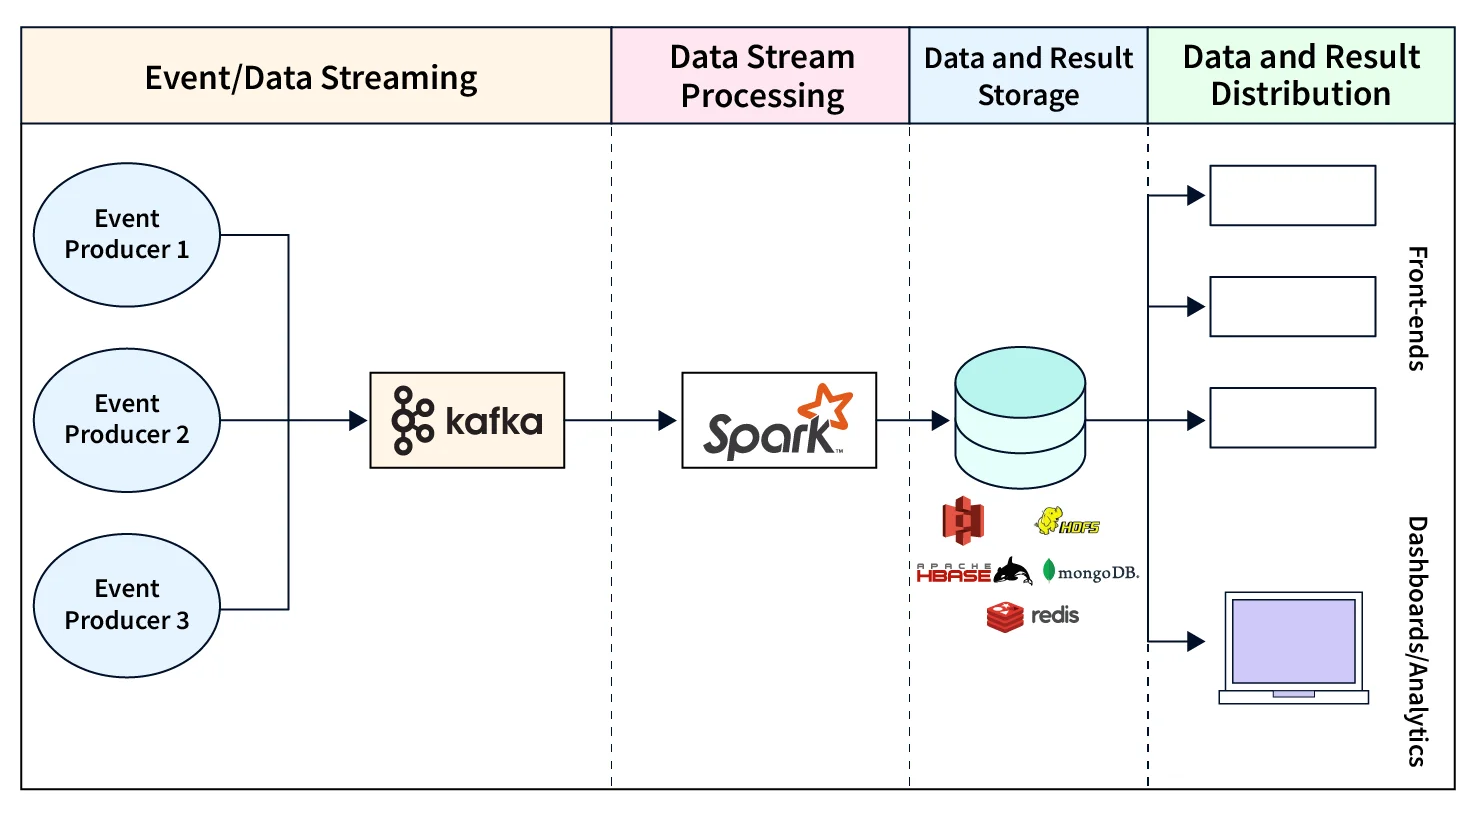
\includegraphics[width=0.7\linewidth]{images/architecture.png} \\
    {\fontsize{5}{6}\selectfont \mbox{\url{https://www.scaler.com/topics/spark-streaming-with-kafka/}}}
\end{center}
\end{frame}


% Mensajería distribuida
\section{Mensajería distribuida}

\begin{frame}
\frametitle{Mensajería distribuida - De picos a flujo estable}
\begin{itemize}
  \item \textbf{Los eventos no se producen a un ritmo constante}
  \begin{itemize}
    \item Sin una infraestructura intermedia el sistema colapsa
    \item Existen picos de carga y consumidores lentos
    \item Las fuentes de datos emiten a ritmo irregular
    \item Los consumidores no pueden ir sincronizados
  \end{itemize}

  \vspace{1em}

  \item \textbf{Middleware Orientado a Mensajes (MOM)}
  \begin{itemize}
    \item Infraestructura intermedia que absorbe picos y reparta trabajo
  \end{itemize}
\end{itemize}
\end{frame}


\begin{frame}
\frametitle{Mensajería distribuida - De P2P a EDA}
\begin{columns}
  \begin{column}{0.55\textwidth}
    \begin{itemize}
      \item \textbf{Integración punto a punto (P2P)}
      \begin{itemize}
        \item Muchas conexiones directas suponen un acoplamiento fuerte
        \item Cambios en contratos y formato implican integraciones frágiles
        \item Cada nuevo consumidor depende excesivamente de los productores
      \end{itemize}

      \vspace{1em}

      \item \textbf{Arquitectura dirigida por eventos (EDA)}
      \begin{itemize}
        \item Productor $\rightarrow$ Distribuidor $\rightarrow$ Consumidor
        \item Productores y consumidores se encuentran desacoplados
        \item Añadir consumidores no implica cambiar productores
      \end{itemize}
    \end{itemize}
  \end{column}

  \begin{column}{0.4\textwidth}
    \centering
    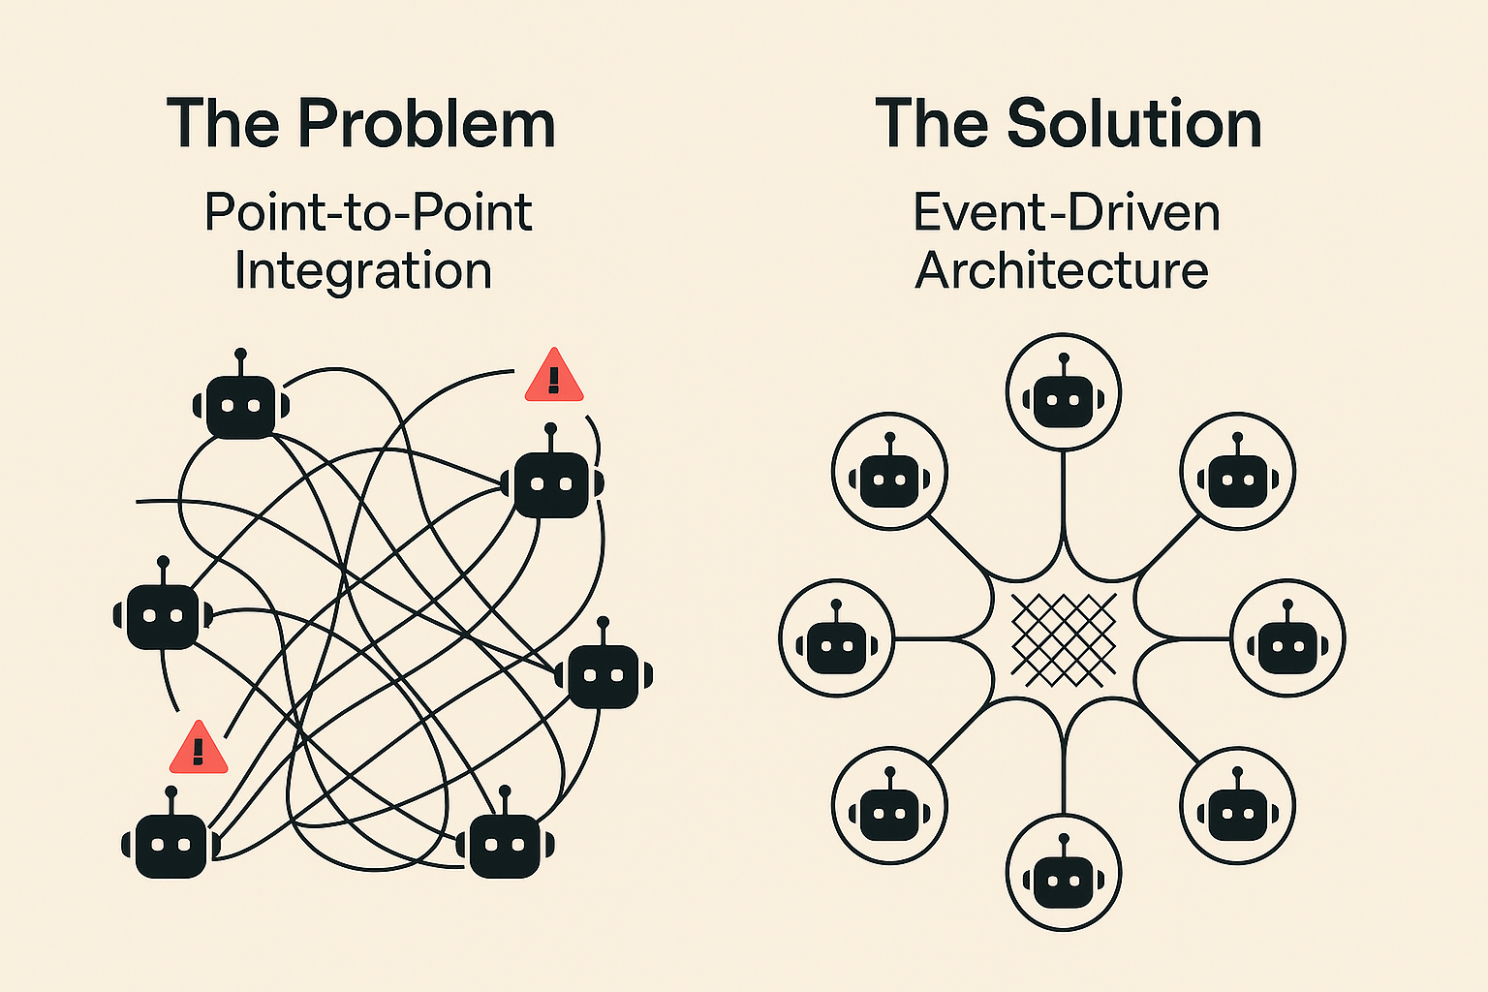
\includegraphics[width=\textwidth]{images/p2peda.png}

    \vspace{1em}
  
    {\fontsize{5}{6}\selectfont \url{https://solace.com/blog/agentic-ai-the-new-microservices/}}
  \end{column}
\end{columns}
\end{frame}

\begin{frame}
\frametitle{Mensajería distribuida - Arquitectura dirigida por eventos}
\begin{itemize}
  \item \textbf{Infraestructura de eventos para datos en movimiento}
  \begin{itemize}
    \item Ingiere, retiene y distribuye eventos de forma desacoplada
    \item Absorbe picos mediante buffering y controles de carga
    \item Fuentes $\rightarrow$ Analítica en vivo $\rightarrow$ Histórico
  \end{itemize}

  \vspace{1em}

  \item \textbf{Sistemas de mensajería distribuida para eventos}
\end{itemize}
\end{frame}


\begin{frame}
\frametitle{Mensajería distribuida - Mensaje vs evento}
\begin{itemize}
  \item \textbf{Un mensaje es el ``sobre`` que transporta un evento}
  \begin{itemize}
    \item Unidad de comunicación $\rightarrow$ payload + headers
    \item Foco en entrega $\rightarrow$ ack, routing, reintentos y colas
  \end{itemize}

  \vspace{1em}

  \item \textbf{Un evento tiene un significado en el dominio}
  \begin{itemize}
    \item Algo ocurrió (quién, qué, cuándo) + contexto
    \item Foco en significado $\rightarrow$ métricas, alertas y reconstrucción de historia
  \end{itemize}

  \vspace{1em}

  \item \textbf{Se transportan eventos dentro del payload de un mensaje}
\end{itemize}
\end{frame}


\begin{frame}
\frametitle{Mensajería distribuida - Patrones de mensajería}
\begin{columns}
  \begin{column}{0.5\textwidth}
    \begin{itemize}
      \item \textbf{Cola de mensajes (Queue)}
      \begin{itemize}
        \item Un evento lo procesa un único consumidor
        \item Útil para tareas y reparto de carga
      \end{itemize}

      \vspace{1em}

      \item \textbf{Publicación/Suscripción (Pub/Sub)}
      \begin{itemize}
        \item Un evento lo reciben muchos consumidores (fan-out)
        \item Útil para métricas + alertas + persistencia en paralelo
      \end{itemize}
    \end{itemize}
  \end{column}

  \begin{column}{0.45\textwidth}
    \centering
    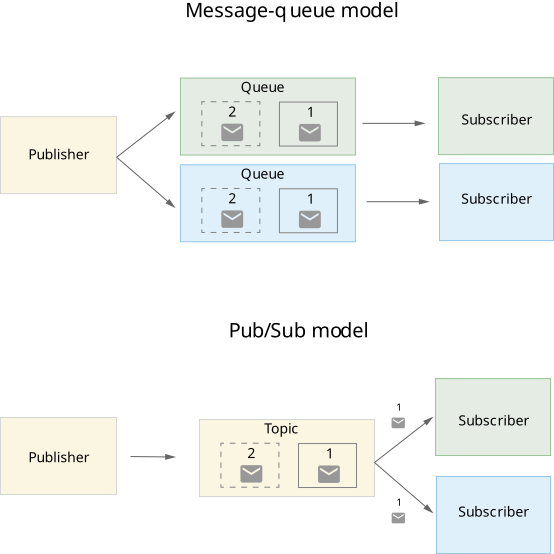
\includegraphics[width=0.8\textwidth]{images/queue_pubsub.png}

    \vspace{1em}
  
    {\fontsize{5}{6}\selectfont \url{https://docs.cloud.google.com/solutions/event-driven-architecture-pubsub}}
  \end{column}
\end{columns}
\end{frame}


\begin{frame}
\frametitle{Mensajería distribuida - Desorden y retardos}
\begin{itemize}
  \item \textbf{Los mensajes no siempre llegan en orden ni en tiempo}
  \begin{itemize}
    \item Latencia en red, buffering y dispositivos que se desconectan y vuelven
    \item Algunas métricas son provisionales y se corrigen si llega un evento tarde
  \end{itemize}

  \vspace{1em}

  \item \textbf{El sistema de mensajería debe tolerar desorden y retardos}
  
  \vspace{1em}

  \item \textbf{Se debe decidir entre perder eventos o tolerar duplicados}
\end{itemize}
\end{frame}


\begin{frame}
\frametitle{Mensajería distribuida - Semánticas de entrega}
\begin{itemize}
  \item \textbf{At-most-once}
  \begin{itemize}
    \item Más rápido $\Rightarrow$ mínima latencia y overhead
    \item Menos fiable $\Rightarrow$ puede perder mensajes
  \end{itemize}

  \vspace{0.5em}

  \item \textbf{At-least-once}
  \begin{itemize}
    \item Más fiable $\Rightarrow$ entrega una o más veces
    \item Más lento $\Rightarrow$ más overhead/latencia
  \end{itemize}

  \vspace{0.5em}

  \item \textbf{Exactly-once}
  \begin{itemize}
    \item Mismo resultado final (efecto único)
    \item No significa ``cero duplicados en la red''
    \item Suele ser más lento y depende de la plataforma
  \end{itemize}
\end{itemize}
\end{frame}

\begin{frame}
\frametitle{Mensajería distribuida - Conceptos clave}
\begin{itemize}
  \item \textbf{Todo sistema de mensajería gestiona cuatro aspectos clave}
  \begin{itemize}
    \item Canales para organizar mensajes en colas, topics o streams
    \item Escalado y paralelismo mediante particiones o consumidores
    \item Fiabilidad mediante acks, reintentos y persistencia
    \item Consumo destructivo tras ack o replay histórico
  \end{itemize}

  \vspace{1em}

  \item \textbf{Cada sistema los prioriza e implementa de forma distinta}
\end{itemize}
\end{frame}


\begin{frame}
\frametitle{Mensajería distribuida - Brokers vs events logs}
\begin{itemize}
  \item \textbf{Brokers clásicos}
  \begin{itemize}
    \item Optimiza la entrega por mensaje
    \item \textit{Smart broker} $\rightarrow$ más lógica y decisiones en el broker
  \end{itemize}

  \vspace{1em}

  \item \textbf{Events logs}
  \begin{itemize}
    \item Optimiza retención, offsets y replay del flujo de eventos
    \item \textit{Dumb broker, smart consumer} $\rightarrow$ más lógica y decisiones en consumidores
  \end{itemize}

  \vspace{1em}

  \item \textbf{Tareas y routing vs histórico, fan-out y reproceso}
\end{itemize}
\end{frame}


\begin{frame}
\frametitle{Mensajería distribuida - Brokers clásicos}
\begin{columns}
  \begin{column}{0.65\textwidth}
    \begin{itemize}
      \item \textbf{Optimiza entrega y routing por mensaje}
      \begin{itemize}
        \item Colas y pub/sub con routing flexible (topics/keys/exchanges)
        \item Patrones de integración habituales (filtering, routing, request/reply)
      \end{itemize}

      \vspace{0.5em}

      \item \textbf{Poseen una alta fiabilidad operativa}
      \begin{itemize}
        \item Acks y reintentos, control de redelivery
        \item Dead-letter queues y políticas de error
      \end{itemize}

      \vspace{0.5em}

      \item \textbf{Ideal para mensajes/tareas asíncronas e integración empresarial}
      \begin{itemize}
        \item Ejemplos incluyen RabbitMQ, ActiveMQ, Amazon SQS, ...
      \end{itemize}
    \end{itemize}
  \end{column}

  \begin{column}{0.3\textwidth}
    \centering
    
\includegraphics[width=0.9\textwidth]{images/rabbitmq.png}

    \vspace{2em}

    
\includegraphics[width=0.45\textwidth]{images/sqs.png}
  \end{column}
\end{columns}
\end{frame}


\begin{frame}
\frametitle{Mensajería distribuida - Events logs}
\begin{columns}
  \begin{column}{0.75\textwidth}
    \begin{itemize}
      \item \textbf{Optimiza el flujo de eventos como un log distribuido}
      \begin{itemize}
        \item Append-only (commit log) con retención (por tiempo/tamaño)
        \item Lectura por offsets $\rightarrow$ cada consumidor controla su progreso
      \end{itemize}

      \vspace{0.5em}

      \item \textbf{Habilita fan-out, retención y replay}
      \begin{itemize}
        \item Muchos consumidores independientes sobre el mismo flujo
        \item Retención para recomputar vistas, auditoría y nuevos consumidores
      \end{itemize}

      \vspace{0.5em}

      \item \textbf{Ideal para analítica en vivo y pipelines de datos}
      \begin{itemize}
        \item Ejemplos incluyen Kafka, Pulsar, AWS Kinesis, ...
      \end{itemize}
    \end{itemize}
  \end{column}

  \begin{column}{0.225\textwidth}
    \centering
    
\includegraphics[width=1\textwidth]{images/kafka.png}
  \end{column}
\end{columns}
\end{frame}


% Procesamiento en streaming
\section{Procesamiento en streaming}

\begin{frame}
\frametitle{Procesamiento en streaming - Eventos continuos}
\begin{itemize}
  \item \textbf{Streaming procesa flujos continuos de eventos}
  \begin{itemize}
    \item No se trata solo de hacerlo rápido
    \item Se computa sobre un flujo continuo que no termina
  \end{itemize}

  \vspace{1em}

  \item \textbf{Batch es un caso particular de un stream finito}
\end{itemize}
\end{frame}


\begin{frame}
\frametitle{Procesamiento en streaming - Tres dimensiones}
\begin{itemize}
  \item \textbf{Dimensiones clave en el procesamiento en streaming}
  \begin{itemize}
    \item Tiempo $\rightarrow$ ¿Cuándo ocurrió el evento vs cuándo lo proceso?
    \item Estado $\rightarrow$ ¿Necesito recordar el pasado para procesar el presente?
    \item Correctitud $\rightarrow$ ¿Qué garantías doy ante fallos, retrasos y duplicados?
  \end{itemize}

  \vspace{1em}

  \item \textbf{Cada sistema en streaming prioriza unas dimensiones sobre otras}
  
  \vspace{1em}
  
  \item \textbf{Existen diferentes enfoques de procesamiento según estas dimensiones}
\end{itemize}
\end{frame}

\begin{frame}
\frametitle{Procesamiento en streaming - De simple a complejo}
\begin{itemize}
  \item \textbf{Simple Event Processing (SEP)}
  \begin{itemize}
    \item Filtra, enruta y transforma evento a evento
    \item Ejemplos incluyen filtrar posiciones imposibles
  \end{itemize}

  \vspace{0.5em}

  \item \textbf{Event Stream Processing (ESP)}
  \begin{itemize}
    \item Consultas continuas, como ventanas, agregaciones y métricas online
    \item Ejemplos incluyen sprints por jugador en 5 min
  \end{itemize}

  \vspace{0.5em}

  \item \textbf{Complex Event Processing (CEP)}
  \begin{itemize}
    \item Patrones complejos y temporales, como secuencias, correlación y anomalías
    \item Ejemplos incluyen análisis de presión sostenida 
  \end{itemize}
\end{itemize}
\end{frame}


\begin{frame}
\frametitle{Procesamiento en streaming - Stateless vs stateful}
\begin{itemize}
  \item \textbf{Procesamiento sin estado (stateless)}
  \begin{itemize}
    \item Cada evento se procesa de forma independiente
    \item Operaciones típicas incluyen map, filter y enrich
  \end{itemize}

  \vspace{1em}

  \item \textbf{Procesamiento con estado (stateful)}
  \begin{itemize}
    \item El procesamiento depende de eventos previos
    \item Operaciones típicas incluyen agregaciones, joins, sesiones y ventanas
  \end{itemize}

  \vspace{1em}

  \item \textbf{El estado introduce complejidad en el sistema}
\end{itemize}
\end{frame}

\begin{frame}
\frametitle{Procesamiento en streaming - Tiempo de proceso vs evento}
\begin{columns}
  \begin{column}{0.55\textwidth}
    \begin{itemize}
      \item \textbf{Tiempo de proceso}
      \begin{itemize}
        \item Cuándo el sistema procesa el evento
        \item Es el reloj del sistema
        \item Monitoriza latencia y rendimiento
      \end{itemize}

      \vspace{1em}

      \item \textbf{Tiempo de evento}
      \begin{itemize}
        \item Cuándo ocurrió en el mundo real
        \item Es el reloj del evento
        \item Necesario para métricas correctas
      \end{itemize}

      \vspace{1em}

      \item \textbf{La verdad del juego es el tiempo de evento}
    \end{itemize}
  \end{column}

  \begin{column}{0.4\textwidth}
    \centering
    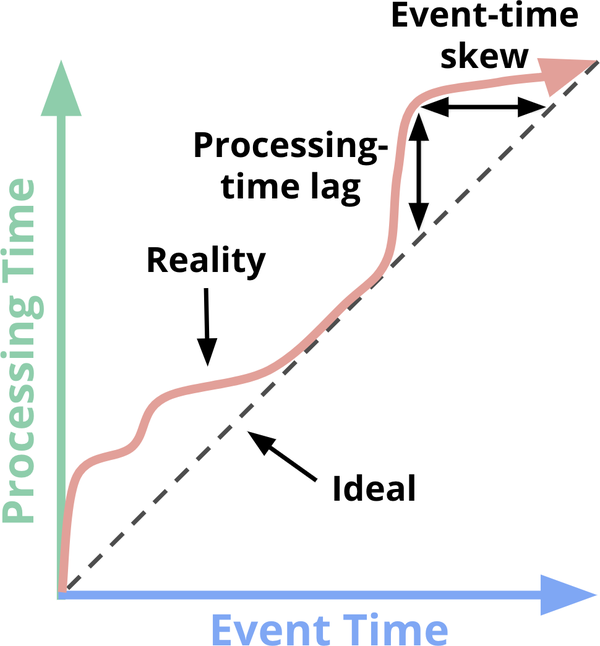
\includegraphics[width=0.75\textwidth]{images/tp_te.png}

    \vspace{1em}
  
    {\fontsize{5}{6}\selectfont Hesse, Guenter. (2022). A benchmark for enterprise stream processing architectures. 10.25932/publishup-56600. }
  \end{column}
\end{columns}
\end{frame}



\begin{frame}
\frametitle{Procesamiento en streaming - Tiempo de proceso vs evento}
\begin{itemize}

  \item \textbf{Alinear el tiempo entre fuentes supone un reto}
  \begin{itemize}
    \item Múltiples fuentes con relojes distintos
    \item Desfases de reloj y necesidad de normalizar timestamps
    \item Retrasos por red, buffering o dispositivos offline
    \item Eventos llegan desordenados o en bloque tras reconexión
  \end{itemize}

  \vspace{1em}

  \item \textbf{Ventanas en tiempo de evento con tolerancia a tardíos}
  \begin{itemize}
    \item Métricas se calculan en tiempo de evento y no de proceso
    \item El sistema acepta tardíos y aplica correcciones con triggers y watermarks
  \end{itemize}
\end{itemize}
\end{frame}



\begin{frame}
\frametitle{Procesamiento en streaming - Ventanas}
\begin{itemize}
  \item \textbf{En flujos continuos no hay un fin definido}
  \begin{itemize}
    \item Para agregar lo infinito se trocea en fragmentos finitos
    \item Se agrupan eventos en ventanas en tiempo de evento
    \item Cada ventana produce un resultado actualizable
  \end{itemize}

  \vspace{1em}

  \item \textbf{El tipo de ventana depende de la pregunta}
  \begin{itemize}
    \item Intervalos fijos, solapados o por inactividad (sesiones)
    \item Es necesario definir tamaño, salto y tolerancia a tardíos
  \end{itemize}
  
  \vspace{1em}
    
  \item \textbf{Mayor correctitud implica mayor complejidad}
\end{itemize}
\end{frame}


\begin{frame}
\frametitle{Procesamiento en streaming - Ventanas}
\begin{columns}
  \begin{column}{0.6\textwidth}
    \begin{itemize}
      \item \textbf{Tumbling}
      \begin{itemize}
        \item Ventanas con segmentos contiguos de tamaño fijo y sin solape
        \item Cada evento cae en una única ventana
      \end{itemize}

      \vspace{0.7em}

      \item \textbf{Hopping/Sliding}
      \begin{itemize}
        \item Ventanas fijas con un salto definido con posible solape
        \item Un evento puede contribuir a varias ventanas
      \end{itemize}

      \vspace{0.7em}

      \item \textbf{Session (por inactividad)}
      \begin{itemize}
        \item Ventanas de tamaño variable delimitadas por un gap sin eventos
        \item Con tardíos, pueden requerir merge de sesiones
      \end{itemize}
    \end{itemize}
  \end{column}

  \begin{column}{0.4\textwidth}
    \centering
    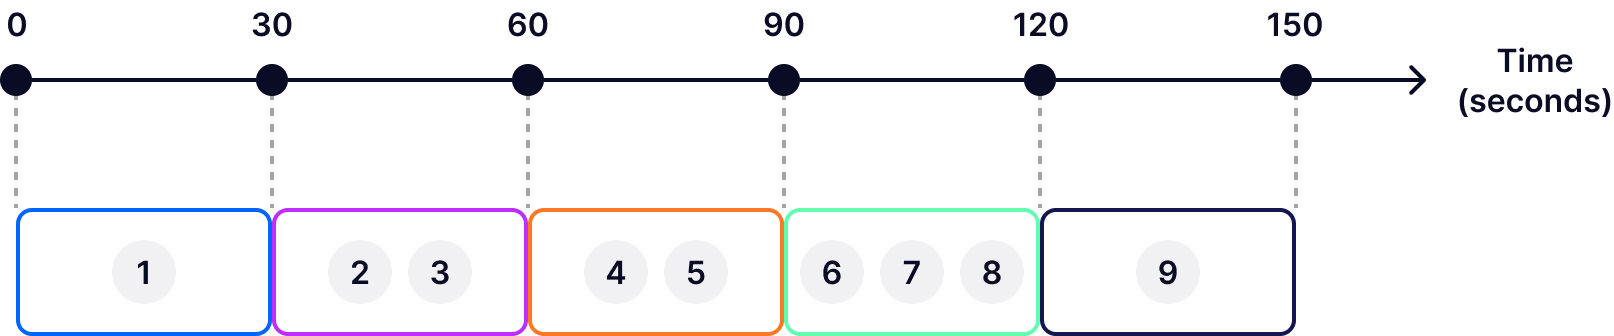
\includegraphics[width=0.8\textwidth]{images/tumbling_windows.png}

    \vspace{1em}
  
    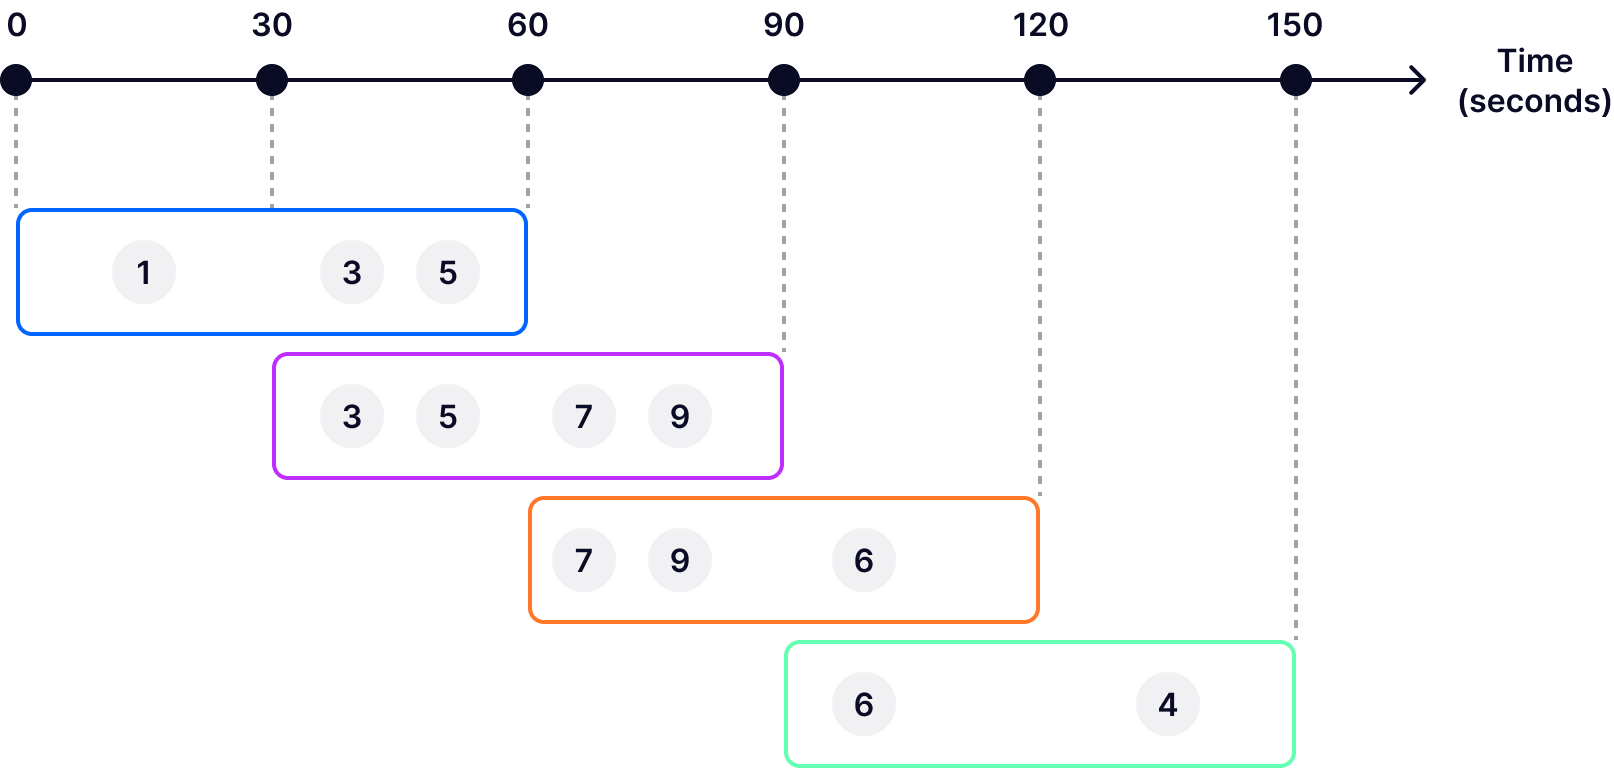
\includegraphics[width=0.8\textwidth]{images/hopping_windows.png}
  
    \vspace{1em}
  
    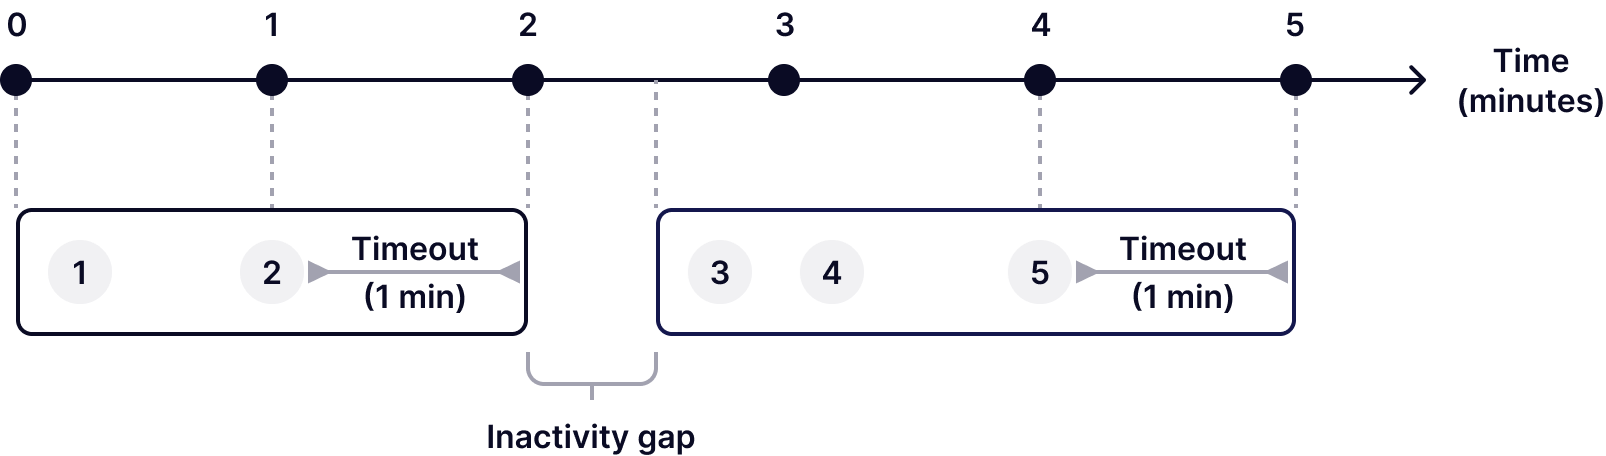
\includegraphics[width=0.8\textwidth]{images/session_windows.png}
  
    \vspace{1em}
  
    {\fontsize{5}{6}\selectfont \url{https://quix.io/blog/windowing-stream-processing-guide}}
  \end{column}
\end{columns}
\end{frame}



\begin{frame}
\frametitle{Procesamiento en streaming - Triggers}
\begin{itemize}

  \item \textbf{Triggers para emitir resultados por ventana}
  \begin{itemize}
    \item Early $\rightarrow$ rápido y aproximado
    \item On-time $\rightarrow$ cuando la ventana se considera completa
    \item Late $\rightarrow$ actualizaciones por eventos tardíos
  \end{itemize}

  \vspace{1em}

  \item \textbf{Streaming involucra resultados revisables}
\end{itemize}
\end{frame}


\begin{frame}
\frametitle{Procesamiento en streaming - Watermarks}
  \begin{itemize}
    \item \textbf{En tiempo de evento los datos pueden llegar tarde y desordenados}

    \vspace{1em}

    \item \textbf{Un watermark indica el progreso del tiempo de evento}
    \begin{itemize}
      \item El sistema necesita una noción de progreso para no esperar indefinidamente
      \item Los eventos con timestamp $<$ watermark se consideran tardíos (late data)
      \item A partir de ese instante asume que eventos más antiguos serán excepcionales
    \end{itemize}

    \vspace{1em}

    \item \textbf{Decide cuándo cerrar ventanas y emitir resultados}
    \begin{itemize}
      \item Agresivo $\rightarrow$ menor latencia, más tardíos y posibles correcciones
      \item Conservador $\rightarrow$ más completitud/exactitud, mayor latencia y más estado
    \end{itemize}
  \end{itemize}
\end{frame}



\begin{frame}
\frametitle{Procesamiento en streaming - Watermarks}
\begin{itemize}

  \item \textbf{Se debe definir hasta cuándo se aceptan tardíos y correcciones}
  \begin{itemize}
    \item Para eventos que llegan con timestamp $<$ watermark
    \item Se define un trade-off entre latencia, coste y exactitud
  \end{itemize}

  \vspace{1em}

  \item \textbf{Políticas de late data más habituales}
  \begin{itemize}
    \item Ignorar/descartar $\rightarrow$ menor coste pero pérdida de exactitud
    \item Emitir correcciones $\rightarrow$ resultados actualizables pero mayor cómputo
    \item Retener estado más tiempo $\rightarrow$ acepta tardíos pero requiere más estado
  \end{itemize}
\end{itemize}
\end{frame}


\begin{frame}
\frametitle{Procesamiento en streaming - Micro-batches vs nativo}
\begin{columns}
  \begin{column}{0.6\textwidth}
    \begin{itemize}
      \item \textbf{Micro-batches}
      \begin{itemize}
        \item Acumula eventos durante un intervalo y los procesa como bloque
        \item Simplifica fallos y permite obtener un alto throughput
      \end{itemize}

      \vspace{1em}

      \item \textbf{Streaming nativo}
      \begin{itemize}
        \item Procesa de forma continua evento a evento
        \item Menor latencia y carga más uniforme sin esperas por lotes
      \end{itemize}

      \vspace{1em}

      \item \textbf{Throughput y simplicidad vs latencia mínima}
    \end{itemize}
  \end{column}

  \begin{column}{0.35\textwidth}
    \centering
    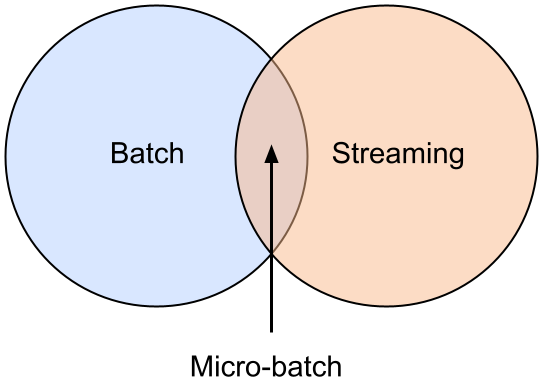
\includegraphics[width=\textwidth]{images/microbatch.png}
  \end{column}
\end{columns}
\end{frame}


\begin{frame}
\frametitle{Procesamiento en streaming - Micro-batches}
\begin{columns}
  \begin{column}{0.6\textwidth}
    \begin{itemize}
      \item \textbf{Optimiza throughput y simplicidad operativa}
      \begin{itemize}
        \item Trata el stream como secuencia de mini-datasets finitos
        \item Simplifica recuperación ante fallos y checkpointing
      \end{itemize}

      \vspace{0.5em}

      \item \textbf{A menudo integra batch y streaming}
      \begin{itemize}
        \item API similar para batch y streaming
        \item Aprovecha optimizaciones del motor batch
      \end{itemize}

      \vspace{0.5em}

      \item \textbf{Ideal para analítica con latencias bajas}
      \begin{itemize}
        \item Ejemplos incluyen Spark Structured Streaming
      \end{itemize}
    \end{itemize}
  \end{column}

  \begin{column}{0.35\textwidth}
    \centering
    
\includegraphics[width=0.8\textwidth]{images/spark.png}
  \end{column}
\end{columns}
\end{frame}


\begin{frame}
\frametitle{Procesamiento en streaming - Nativo}
\begin{columns}
  \begin{column}{0.6\textwidth}
    \begin{itemize}
      \item \textbf{Optimiza baja latencia evento a evento}
      \begin{itemize}
        \item Procesa eventos de forma continua al llegar
        \item Carga más uniforme sin esperas por lotes
      \end{itemize}

      \vspace{0.5em}

      \item \textbf{Estado de primera clase gestionado por el motor}
      \begin{itemize}
        \item Diseñado para event time, watermarks y estado distribuido
      \end{itemize}

      \vspace{0.5em}

      \item \textbf{Ideal para latencias extremadamente bajas}
      \begin{itemize}
        \item Ejemplos incluyen Apache Flink, Storm
      \end{itemize}
    \end{itemize}
  \end{column}

  \begin{column}{0.3\textwidth}
    \centering
    
\includegraphics[width=0.65\textwidth]{images/flink.png}
  
    \vspace{2em}

    
\includegraphics[width=0.8\textwidth]{images/storm.png}
  \end{column}
\end{columns}
\end{frame}


% Diseño a nivel de sistema
\section{Diseño a nivel de sistema}

\begin{frame}
\frametitle{Diseño del sistema - El reto del tiempo real}
\begin{itemize}
  \item \textbf{Pasar de batch y monolitos a tiempo real distribuido supone un reto}
  \begin{itemize}
    \item Nuevas piezas $\rightarrow$ mensajería distribuida y motor streaming
    \item Nuevas propiedades $\rightarrow$ latencia, estado, tiempo de evento
    \item Nuevas complejidades $\rightarrow$ desorden, tardíos, fallos parciales
  \end{itemize}

  \vspace{1em}

  \item \textbf{El objetivo es equilibrar latencia, throughput y exactitud}
\end{itemize}
\end{frame}

\begin{frame}
\frametitle{Diseño del sistema - Teorema CAP}
\begin{columns}
  \begin{column}{0.55\textwidth}
    \begin{itemize}
      \item \textbf{No es posible garantizar simultáneamente}
      \begin{itemize}
        \item \textbf{C}onsistency $\rightarrow$ todos ven lo mismo a la vez
        \item \textbf{A}vailability $\rightarrow$ el sistema siempre responde
        \item \textbf{P}artition $\rightarrow$ sobrevives a particiones de red
      \end{itemize}

      \vspace{1em}

      \item \textbf{En sistemas distribuidos siempre hay particiones}
      \begin{itemize}
        \item Se debe elegir entre consistency (CP) o availability (AP)
      \end{itemize}
    \end{itemize}
  \end{column}

  \begin{column}{0.4\textwidth}
    \centering
    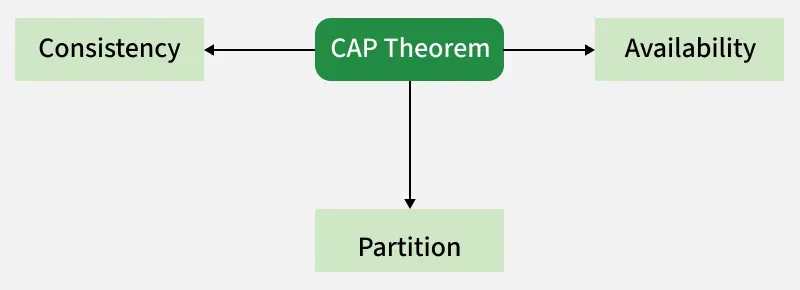
\includegraphics[width=\textwidth]{images/cap_theorem.png}

    \vspace{1em}
  
    {\fontsize{5}{6}\selectfont \url{https://www.geeksforgeeks.org/system-design/cap-theorem-in-system-design/}}
  \end{column}
\end{columns}
\end{frame}

\begin{frame}
\frametitle{Diseño del sistema - CP vs AP}
\begin{itemize}
  \item \textbf{AP prioriza disponibilidad y baja latencia}
  \begin{itemize}
    \item Responder rápido aunque sea con una vista desactualizada
    \item La consistencia eventual puede no estar al milisegundo
  \end{itemize}

  \vspace{1em}

  \item \textbf{CP prioriza consistencia y exactitud}
  \begin{itemize}
    \item Responder coherente aunque sea más lento
    \item Puede bloquear o dar error antes que dar un dato inconsistente
  \end{itemize}

  \vspace{1em}

  \item \textbf{Para analítica en vivo se suele priorizar AP}
\end{itemize}
\end{frame}

\begin{frame}
\frametitle{Diseño del sistema - Arquitectura Lambda}
  \begin{itemize}
    \item \textbf{Idealmente se quiere velocidad y exactitud a la vez}
    \begin{itemize}
      \item Streaming da rapidez pero puede ser aproximado
      \item Batch da precisión pero llega tarde
    \end{itemize}

    \vspace{1em}

    \item \textbf{Lambda propone dos caminos en paralelo}
    \begin{itemize}
      \item Capa rápida para resultados inmediatos
      \item Capa batch para corregir el histórico
    \end{itemize}

    \vspace{1em}

    \item \textbf{El usuario ve resultados rápidos que se refinan con el tiempo}
  \end{itemize}
\end{frame}

\begin{frame}
\frametitle{Diseño del sistema - Arquitectura Lambda}
\begin{itemize}
  \item \textbf{Speed layer para procesamiento en tiempo real}
  \begin{itemize}
    \item Eventos recientes con baja latencia
    \item Puede ser aproximado o tener gaps
  \end{itemize}

  \vspace{1em}

  \item \textbf{Batch layer para reproceso del histórico completo}
  \begin{itemize}
    \item Recalcula todo desde el principio periódicamente
    \item Resultados exactos y completos pero que tardan más
  \end{itemize}

  \vspace{1em}

  \item \textbf{Serving layer para combinar ambas vistas}
  \begin{itemize}
    \item Speed para lo reciente + batch para el histórico corregido
  \end{itemize}
\end{itemize}
\end{frame}

\begin{frame}
\frametitle{Diseño del sistema - Arquitectura Lambda}
\begin{center}
    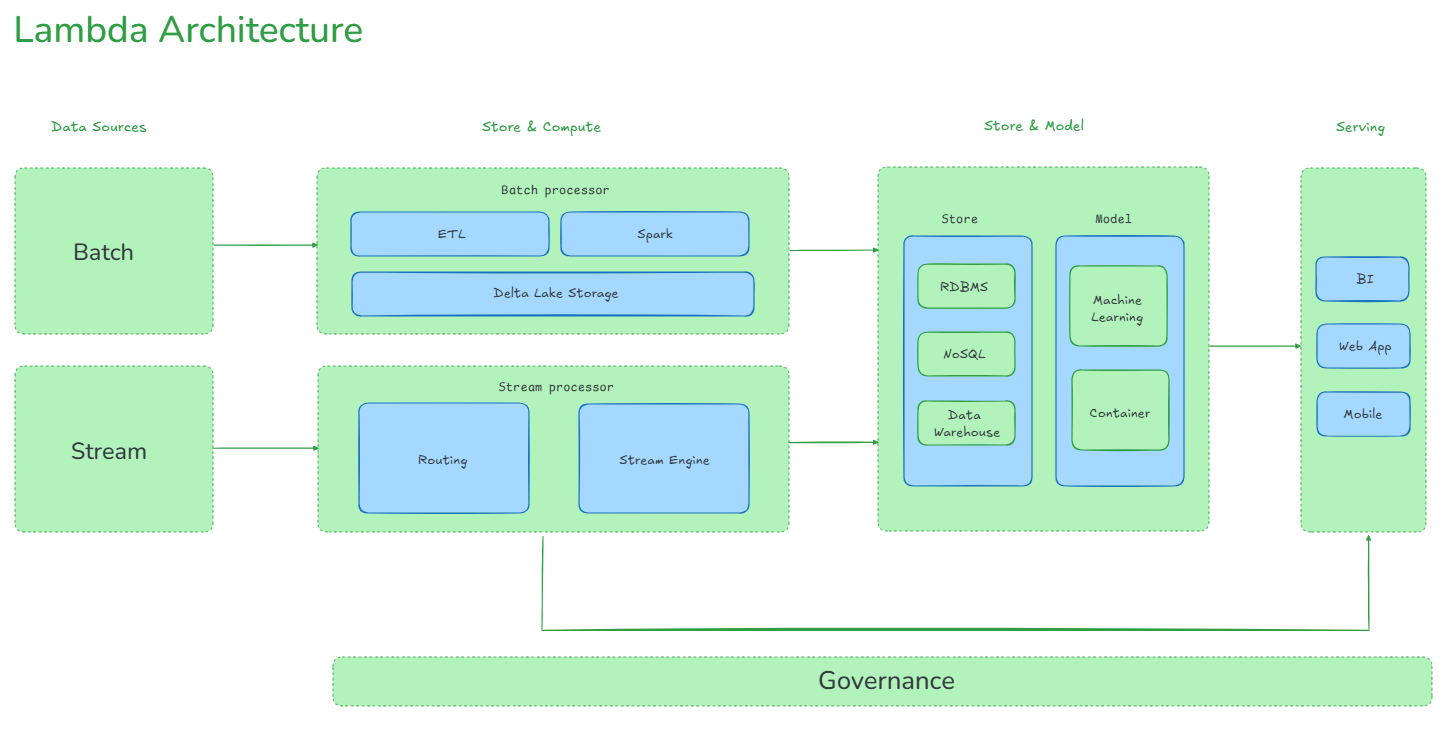
\includegraphics[width=0.8\textwidth]{images/lambda_architecture.png}
    {\fontsize{5}{6}\selectfont \url{https://www.chaosgenius.io/blog/lambda-architecture/}}
\end{center}
\end{frame}

\begin{frame}
\frametitle{Diseño del sistema - Arquitectura Lambda}
\begin{itemize}
  \item \textbf{Proporciona velocidad y exactitud}

  \vspace{1em}

  \item \textbf{Supone una alta complejidad operativa}
  \begin{itemize}
    \item Dos sistemas separados para batch y streaming
    \item Misma lógica implementada dos veces
    \item Difícil depurar cuando no coinciden los resultados
  \end{itemize}

  \vspace{1em}

  \item \textbf{Lambda no vence el teorema CAP}
\end{itemize}
\end{frame}


\begin{frame}
\frametitle{Diseño del sistema - Arquitectura Kappa}
  \begin{itemize}

    \item \textbf{En Kappa todo es streaming}
    \begin{itemize}
      \item Un solo motor para procesar eventos
      \item Batch es simplemente un stream acotado con inicio y fin
    \end{itemize}

    \vspace{1em}

    \item \textbf{Simplifica con un solo camino y una sola lógica}
  \end{itemize}
\end{frame}

\begin{frame}
\frametitle{Diseño del sistema - Arquitectura Kappa}
\begin{itemize}
  \item \textbf{Log persistente como fuente de verdad}
  \begin{itemize}
    \item El sistema de mensajería conserva eventos
    \item El motor de streaming lee desde el log
  \end{itemize}

  \vspace{1em}

  \item \textbf{Procesamiento único con replay cuando se necesita}
  \begin{itemize}
    \item Normalmente procesa eventos en tiempo real
    \item Si hay que recalcular lee el log desde el principio (replay)
  \end{itemize}

  \vspace{1em}

  \item \textbf{El motor de streaming procesa en vivo y reprocesa con replay}
\end{itemize}
\end{frame}

\begin{frame}
\frametitle{Diseño del sistema - Arquitectura Kappa}
\begin{center}
    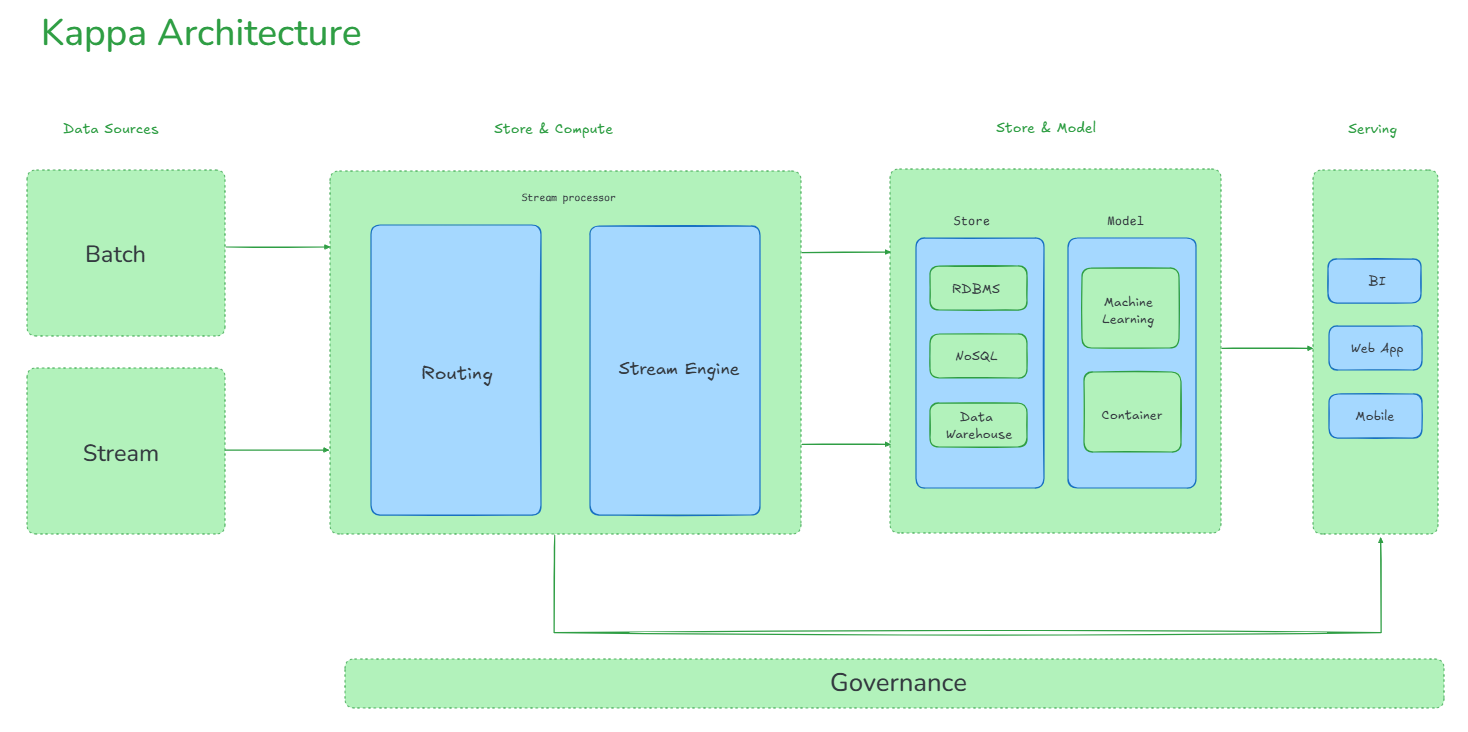
\includegraphics[width=0.8\textwidth]{images/kappa_architecture.png}
    {\fontsize{5}{6}\selectfont \url{https://www.chaosgenius.io/blog/kappa-architecture/}}
\end{center}
\end{frame}

\begin{frame}
\frametitle{Diseño del sistema - Arquitectura Kappa}
\begin{itemize}
  \item \textbf{Si se descubre un error en el procesamiento}
  \begin{itemize}
    \item Se corrige la lógica y se lanza un nuevo proceso
    \item El proceso lee el log completo desde el principio
    \item Procesa todo a máxima velocidad hasta alcanzar el presente
    \item Se sustituye el proceso antiguo por el nuevo
  \end{itemize}

  \vspace{1em}

  \item \textbf{Se requiere un log persistente y un motor streaming robusto}
\end{itemize}
\end{frame}

\begin{frame}
\frametitle{Diseño del sistema - Desafíos en producción}
\begin{itemize}

  \item \textbf{Elegir entre Lambda o Kappa no es suficiente}

  \vspace{1em}

  \item \textbf{Existen múltiples aspectos clave a considerar}
  \begin{itemize}
    \item ¿Cómo servir los datos según cada necesidad? (serving)
    \item ¿Cómo operar el sistema en producción? (fiabilidad)
    \item ¿Cómo garantizar calidad de datos en tiempo real?
    \item ¿Cómo proteger privacidad y definir accesos?
  \end{itemize}

\end{itemize}
\end{frame}

\begin{frame}
\frametitle{Diseño del sistema - Serving deportivo}
\begin{itemize}
  \item \textbf{Un mismo evento tiene diferentes vistas según el uso}

  \vspace{0.6em}

  \item \textbf{Dashboard en vivo (hot)}
  \begin{itemize}
    \item KPIs por ventana (1--3 min) + alertas inmediatas
  \end{itemize}

  \vspace{0.6em}

  \item \textbf{Histórico para ML y análisis (cold)}
  \begin{itemize}
    \item Dataset curado para entrenar y validar modelos
  \end{itemize}
\end{itemize}
\end{frame}


\begin{frame}
\frametitle{Diseño del sistema - Fiabilidad del sistema}
\begin{itemize}
  \item \textbf{El sistema debe manejar picos y fallos}
  \begin{itemize}
    \item Durante un partido ocurren muchos eventos simultáneos
    \item Si algo falla el sistema debe recuperar sin perder datos
  \end{itemize}

  \vspace{1em}

  \item \textbf{Existen diferentes métricas clave a vigilar}
  \begin{itemize}
    \item ¿Existen retrasados? (lag)
    \item ¿Los datos llegan a tiempo? (latencia)
    \item ¿Se están perdiendo eventos? (errores)
  \end{itemize}

  \vspace{1em}

  \item \textbf{Si el sistema se satura se debe escalar o priorizar eventos}
\end{itemize}
\end{frame}

\begin{frame}
\frametitle{Diseño del sistema - Calidad del dato}
\begin{itemize}
  \item \textbf{En streaming no se puede parar para limpiar}
  \begin{itemize}
    \item Se necesitan reglas claras de calidad
    \item El sistema debe seguir funcionando con datos imperfectos
  \end{itemize}

  \vspace{1em}

  \item \textbf{Se requiere validación y limpieza en tiempo real}
  \begin{itemize}
    \item Eventos malformados van a cuarentena (dead-letter queue)
    \item Deduplicar eventos repetidos por ID
    \item Validar esquemas y compatibilidad
  \end{itemize}

  \vspace{1em}

  \item \textbf{El reto no es solo ser rápido sino también coherente}
\end{itemize}
\end{frame}



\begin{frame}
\frametitle{Diseño del sistema - Privacidad y ética}
\begin{itemize}
  \item \textbf{Es necesario definir quién accede a qué datos}
  \begin{itemize}
    \item Diferentes roles con distintos permisos
    \item Datos agregados vs datos individuales
  \end{itemize}

  \vspace{1em}

  \item \textbf{Existen diferentes preguntas clave}
  \begin{itemize}
    \item ¿Quién puede ver qué? (staff, analistas, médicos)
    \item ¿Para qué se usa? (rendimiento, prevención, investigación)
    \item ¿Cuánto tiempo se guarda? (retención y borrado)
  \end{itemize}

  \vspace{1em}
  \item \textbf{Se deben definir responsabilidades y límites}
\end{itemize}
\end{frame}

\begin{frame}
\frametitle{Conclusiones}
\begin{itemize}
  \item \textbf{Elección de arquitectura según necesidades}
  \begin{itemize}
    \item Batch si latencia no importa (reportes diarios)
    \item Streaming si necesitas reaccionar rápido (alertas en vivo)
    \item Lambda (robusta, dos caminos) vs Kappa (simple, un camino con replay)
  \end{itemize}

  \vspace{1em}

  \item \textbf{Streaming consta de mensajería + motor + serving}
  \begin{itemize}
    \item Mensajería que desacopla fuentes y consumidores
    \item Motor streaming procesa con posible estado y ventanas de tiempo
    \item Serving genera vistas hot (alertas en vivo) y cold (ML e histórico)
  \end{itemize}

  \vspace{1em}

  \item \textbf{Trade-offs inevitables son velocidad vs exactitud vs complejidad}
\end{itemize}
\end{frame}

\end{document}
